\documentclass{article}
\usepackage{graphicx}
\usepackage{mathtools}
\usepackage{amsfonts}
\usepackage{ngerman}
\usepackage{hyperref}
\usepackage{natbib}
\usepackage{rotating}
\usepackage[table, dvipsnames, usenames]{xcolor}
\usepackage{color}
\usepackage[justification=centering]{caption}
\usepackage{float}
\usepackage{subcaption}
\usepackage{caption}
\usepackage{array}
\newcolumntype{C}[1]{>{\centering\let\newline\\\arraybackslash\hspace{0pt}}m{#1}}



\begin{document}

\section{bla bla bla Mr. Freeman}

\begin{table}
\begin{center}


\caption{Diese Tabelle zeigt die Strukturen der $\alpha$-Proteine der Fallstudie. Alle Proteine dieser Tabelle geh\"oren zur Architektur der \textit{Up down Bundles}. Die Bilder der 3D-Strukturen und die Beschreibunng der Eintr\"age stammen aus der PDB. Die Einordnung der Topologie und der Superfamilie stammt aus CATH. }
\begin{tabular}{ | C{9mm} | C{30mm} | C{29mm} | C{38mm} | }
\hline
PDB-ID & 3D Bild & Struktur & Beschreibung \\ \hline
1QPU  & 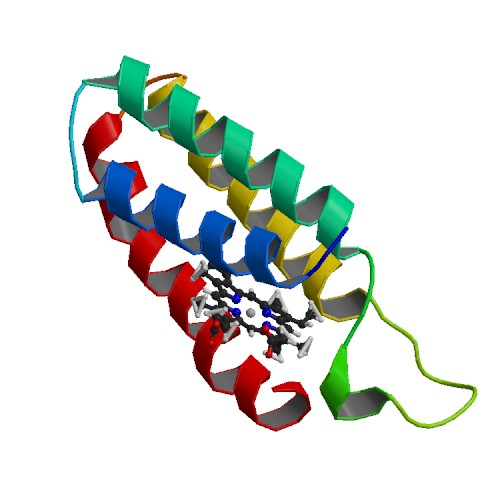
\includegraphics[width=30mm, trim= -10 -5 -5 -10]{1QPU_asym_r_500.jpg} & Topologie: \newline \textit{Four Helix Bundle} \newline Superfamilie: CATH: 1.20.120.10 & Der Eintrag beschreibt die Struktur des oxidierten Cytochrom B562 aus \textit{E. coli} \cite{1qpu}. Es ist am Elektronentransport beteiligt. \\ \hline
1QQ3  & 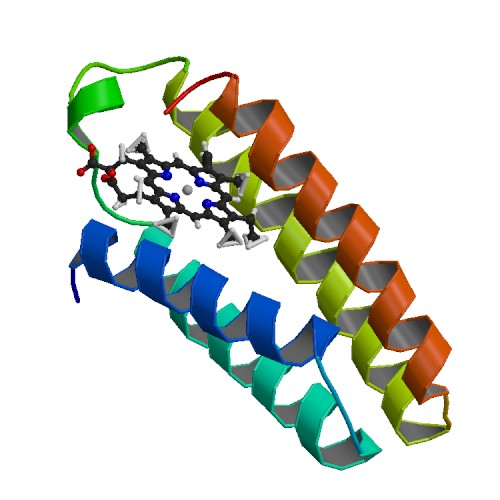
\includegraphics[width=30mm, trim= -10 -5 -5 -10]{1QQ3_asym_r_500.jpg} & Topologie: \newline \textit{Four Helix Bundle} \newline Superfamilie: CATH: 1.20.120.10  & Die Hem-bindende Variante des oxidierten Cytochrom B562 aus \textit{E. coli} wird durch diesen Eintrag beschrieben \cite{1qq3}. Auch diese Variante des Proteins ist f\"ur Elektronentransport zust\"andig. \\ \hline
1CGN  & 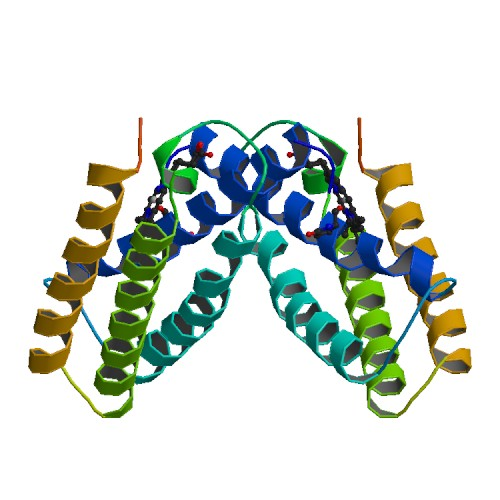
\includegraphics[width=30mm, trim= -10 -5 -5 -10]{1CGN_bio_r_500.jpg} & Topologie: \newline \textit{Four Helix Bundle} \newline Superfamilie: CATH: 1.20.120.10  & Dieser Eintrag beschreibt die Struktur von Cytochrom C' \cite{1cgn} aus \textit{Achromobacter xylosoxidans}. Es ist ebenfalls f\"ur Elektronentransport zust\"andig. \\ \hline
1HE9  & 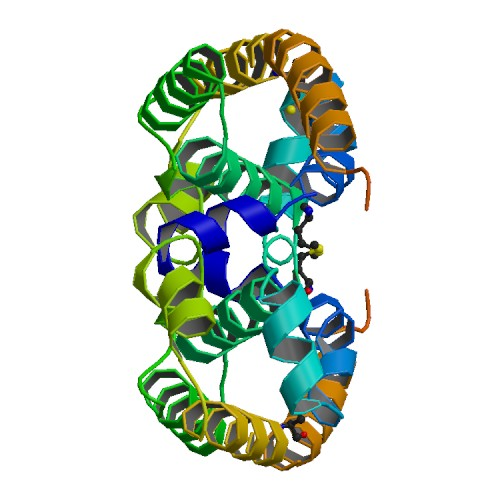
\includegraphics[width=30mm, trim= -10 -5 -5 -10]{1HE9_bio_r_500.jpg}  & Topologie: \newline \textit{Four Helix Bundle} \newline Superfamilie: \newline \textit{Bacterial GAP Domain}   & Der Eintrag beschreibt die GTPase aktivierende Dom\"ane des Toxins Exoenzyms S aus \textit{Pseudomonas aeruginosa} \cite{1he9}. \\ \hline
3GF9  & 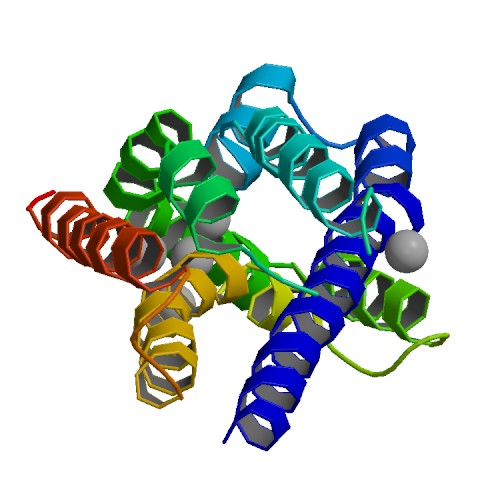
\includegraphics[width=30mm, trim= -10 -5 -5 -10]{3GF9_bio_r_500.jpg} & Topologie: \newline \textit{Dbl homology Domain} \newline Superfamilie: \newline DBL Homology Domain & Die RhoGEF-Dom\"ane des  Proteins Intersectin 2 aus \textit{Homo sapiens} wird durch den Eintrag 3GF9 beschrieben \cite{3gf9}. Dieses Protein ist f\"ur Endocytose zust\"andig. \\ 
\hline

\end{tabular}
\end{center}
\end{table}


\begin{table}
\begin{center}
\caption{Diese Tabelle zeigt die Strukturen der $\beta$-Proteine der Fallstudie. Alle Proteine in dieser Tabelle geh\"oren zur Architektur der $\beta$-\textit{Barrels}. Die Bilder der 3D-Strukturen und die Beschreibunng der Eintr\"age stammen aus der PDB. Die Einordnung der Topologie und der Superfamilie stammt aus CATH. }
\begin{tabular}{ | C{9mm} | C{30mm} | C{29mm} | C{38mm} | }
\hline
PDB-ID & 3D Bild & Struktur & Beschreibung \\ \hline
1EXS  & 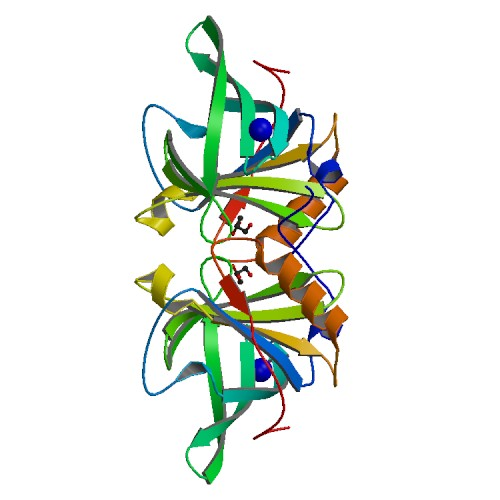
\includegraphics[width=30mm, trim= -10 -5 -5 -10]{1EXS_bio_r_500.jpg} & Topologie: \newline \textit{Lipocalin} \newline Superfamilie: CATH: 2.40.128.20 & Der Eintrag 1EXS beschreibt die Struktur des $\beta$-Lactoglobulin aus \textit{Sus scrofa} \cite{1exs}. Es ist ein lipidbindendes Protein. \\ \hline
1NGL  & 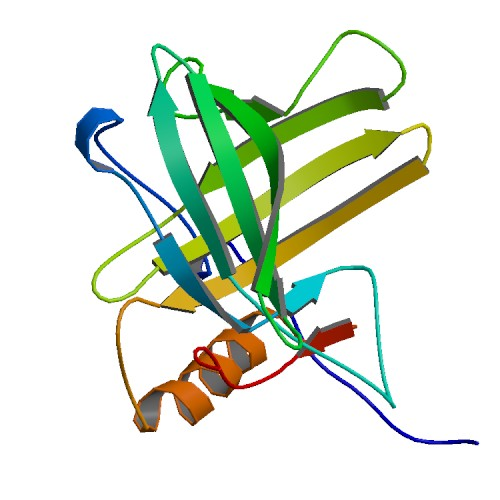
\includegraphics[width=30mm, trim= -10 -5 -5 -10]{1NGL_asym_r_500.jpg} & Topologie: \newline \textit{Lipocalin} \newline Superfamilie: CATH: 2.40.128.20  & Das neutrophile Gelatinase asoziierte Lipocalin des \textit{Homo sapiens} wird durch den Eintrag 1NGL beschrieben \cite{1ngl}. Es ist ein Transportprotein. \\ \hline
1QQS  & 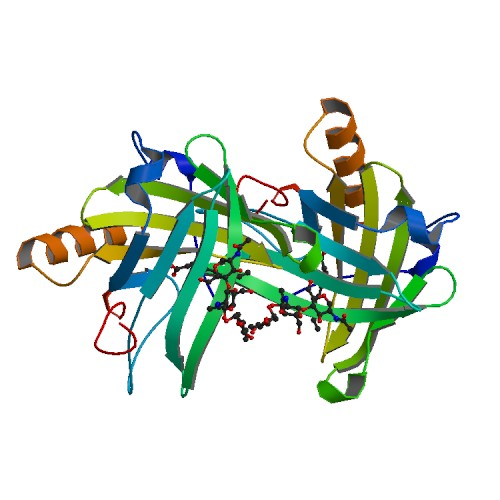
\includegraphics[width=30mm, trim= -10 -5 -5 -10]{1QQS_bio_r_500.jpg} & Topologie: \newline \textit{Lipocalin} \newline Superfamilie: CATH: 2.40.128.20  & Die Struktur des neutrophilen Gelatinase assoziierten Lipocalin Homodimers wird durch den Eintrag 1QQS beschrieben \cite{1qqs}. Es ist ein zuckerbindendes Protein.  \\ \hline
3SLO  & 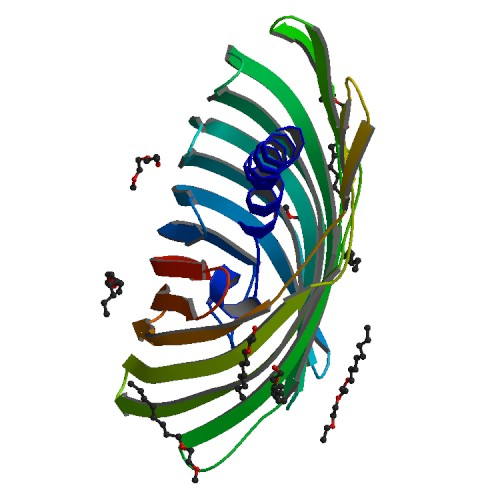
\includegraphics[width=30mm, trim= -10 -5 -5 -10]{3SLO_bio_r_500.jpg}  & Topologie: \newline \textit{Lipocalin} \newline Superfamilie: \newline Autortransporter Esterase   & Der Eintrag 3SLO beschreibt die Struktur der N1023D Mutante des Autotransporters EspP \cite{3slo} aus \textit{E. coli}. Dieses Protein ist f\"ur den Transport von Proteinen zust\"andig. \\ \hline
1WJX  & 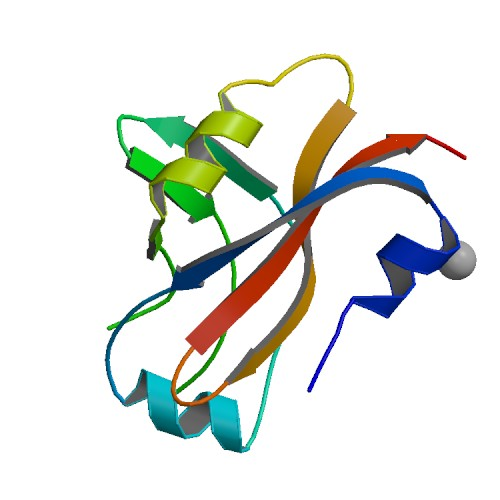
\includegraphics[width=30mm, trim= -10 -5 -5 -10]{1WJX_bio_r_500.jpg} & Topologie: \newline \textit{Small Protein B} \newline Superfamilie: \newline 2.40.280.10 & Dieser Eintrag beschreibt das Protein TT0801 aus \textit{Thermus thermophilus} \cite{1wjx}. \\ 
\hline


\end{tabular}
\end{center}
\end{table}




\begin{table}
\begin{center}
\caption{Hier werden die $\alpha/\beta$-Proteine der Fallstudie gezeigt. Alle hier dargestellten Proteine haben eine \textit{3-Layer-Sandwich}-Architektur. Die Bilder und Beschreibungen entstammen der PDB. Die Beschreibung der Struktur stammt aus CATH.}
\begin{tabular}{ | C{9mm} | C{30mm} | C{29mm} | C{38mm} | }
\hline
PDB-ID & 3D Bild & Struktur & Beschreibung \\ \hline
5CHY  & 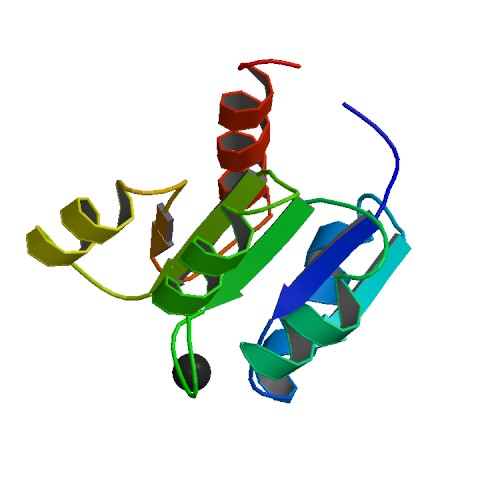
\includegraphics[width=30mm, trim= -10 -5 -5 -10]{5CHY_bio_r_500.jpg} & Topologie: \newline \textit{\textit{Rossman Fold}} \newline Superfamilie: CATH: 3.40.50.2300 & Der Eintrag beschreibt die Struktur einer Mutante des Chemotaxisproteins des Gens \textit{cheY} aus \textit{E. coli} \cite{5chy}. Es ist ein Signaltransduktionsproteinprotein. \\ \hline
2ID9  & 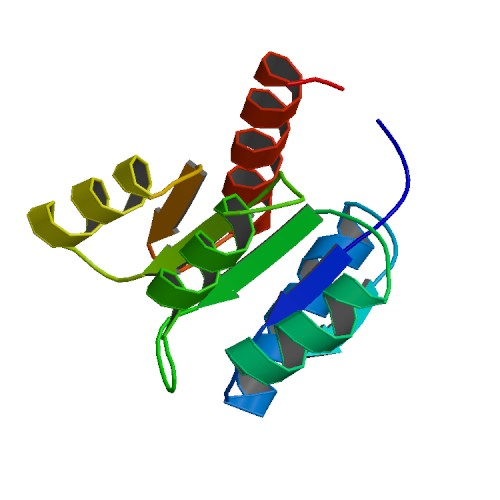
\includegraphics[width=30mm, trim= -10 -5 -5 -10]{2ID9_bio_r_500.jpg} & Topologie: \newline \textit{\textit{Rossman Fold}} \newline Superfamilie: CATH: 3.40.50.2300  & Der Eintrag beschreibt das synthetische Protein T87I phosphono-CheY \cite{2id9}. Es ist ein stabiles Analogon zu dem oben beschriebenen Chemotaxisprotein. \\ \hline
3I42  & 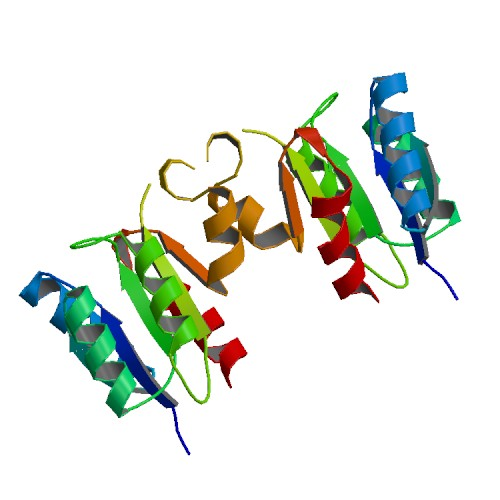
\includegraphics[width=30mm, trim= -10 -5 -5 -10]{3I42_bio_r_500.jpg} & Topologie: \newline \textit{\textit{Rossman Fold}} \newline Superfamilie: CATH: 3.40.50.2300  & Der Eintrag beschreibt eine Empfängerdom\"ane aus \textit{Methylobacillus flagellatus}, die regulatorische Signale empf\"angt und \"ahnlich zu \textit{cheY} ist \cite{3i42}.  \\ \hline
1D4O  & 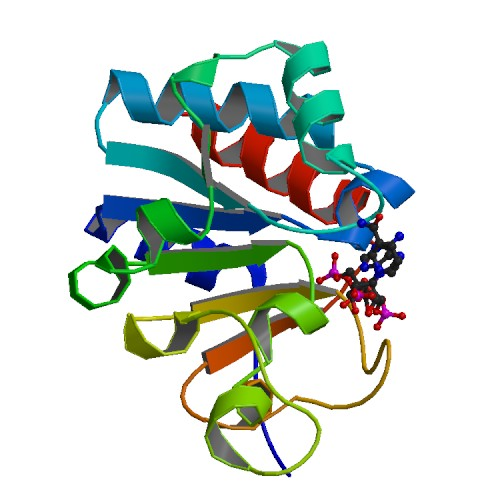
\includegraphics[width=30mm, trim= -10 -5 -5 -10]{1D4O_bio_r_500.jpg}  & Topologie: \newline \textit{Rossman Fold} \newline Superfamilie: \newline \textit{TPP-binding domain} & Die Struktur der Transhydrogenase Dom\"ane II aus \textit{Bos taurus} \cite{1d4o} wird durch diesen Eintrag beschreiben. Sie wird in der PDB als Oxidoreductase klassifiziert. \\ \hline
2W0I  & 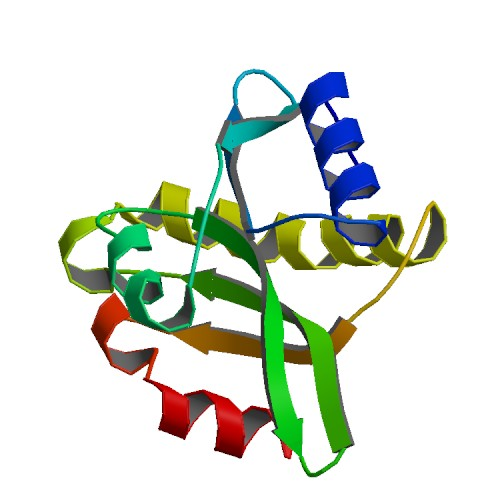
\includegraphics[width=30mm, trim= -10 -5 -5 -10]{2W0I_bio_r_500.jpg} & Topologie: \newline Severin \newline Superfamilie: \newline Severin & Der Eintrag beschreibt eine Dom\"ane des Proteins TWINFLIN-2 aus \textit{Homo sapiens} \cite{2woi}. Dieses Protein inhibiert die Polymerisation von Actin. \\ 
\hline


\end{tabular}
\end{center}
\end{table}

\section{Aldolase}

\begin{table}
\begin{center}
\caption{Aldolasen Teil 1}
\begin{tabular}{ | C{9mm} | C{30mm} | C{29mm} | C{38mm} | }
\hline
PDB-ID & 3D Bild & Struktur & Beschreibung \\ \hline
1LBM  & 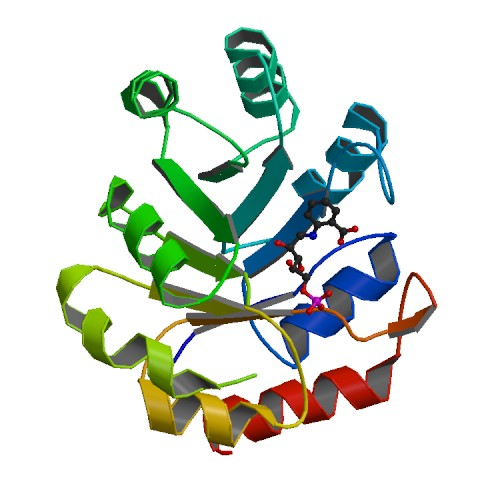
\includegraphics[width=30mm, trim= -10 -5 -5 -10]{1LBM_bio_r_500.jpg} & Topologie: \newline TIM \textit{Barrel} \newline Superfamilie: Aldolasen - Klasse I & Der Eintrag beschreibt die Phosphoribosyl Anthranilat Isomerase im Komplex mit einem Liganden aus \textit{Thermotoga maritima} \cite{1lbm}. Das Protein ist Teil des Stoffewechselweges zur Synthese von L-Tryptophan. \\ \hline
1LOR  & 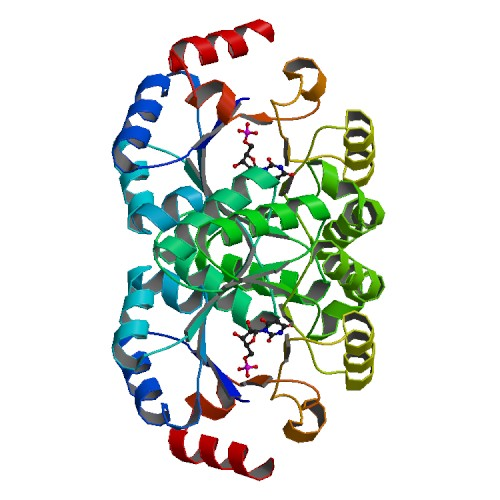
\includegraphics[width=30mm, trim= -10 -5 -5 -10]{1LOR_bio_r_500.jpg} & Topologie: \newline \textit{\textit{Rossman Fold}} \newline Superfamilie: CATH: 3.40.50.2300  & Die Struktur der Orotidin 5'-Monophosphatase aus \textit{Methanothermobacter thermautotrophicus} im Komplex mit einem Liganden wird durch diesen Eintrag beschrieben \cite{1lor}. Das Protein ist an der Decarboxylierung von Oritidin beteiligt. \\ \hline
1MXS  & 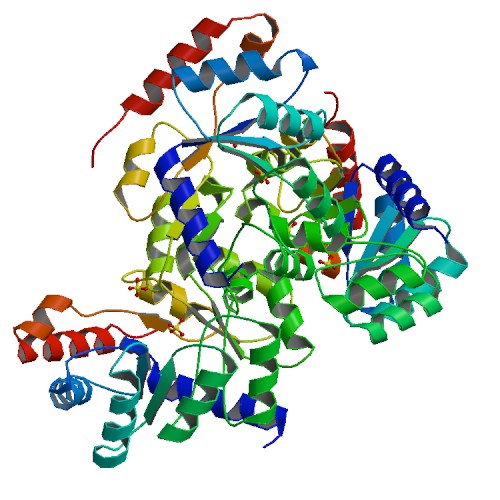
\includegraphics[width=30mm, trim= -10 -5 -5 -10]{1MXS_bio_r_500.jpg} & Topologie: \newline \textit{\textit{Rossman Fold}} \newline Superfamilie: CATH: 3.40.50.2300  & Dieser Eintrag beschreibt die 2-Keto-3-deoxy-6-Phosphogluconat Aldolase aus \textit{Pseudomonas putida} \cite{1mxs}. Genau wie die obigen Proteine wird dieses durch die PDB als Lyase klassifiziert. \\ \hline
1NSJ  & 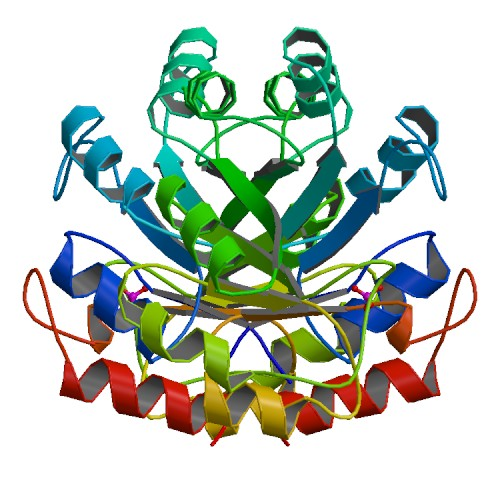
\includegraphics[width=30mm, trim= -10 -5 -5 -10]{1NSJ_bio_r_500.jpg}  & Topologie: \newline \textit{Rossman Fold} \newline Superfamilie: \newline \textit{TPP-binding domain} & Die Struktur der phosphoribosyl Anthranilat Isomerase aus \textit{Thermotoga maritima} wird duch diesen Eintrag beschrieben \cite{1nsj}. Auch dieses Protein ist in die Synthese von L-Tryptophan eingebunden. \\ \hline
1V5X  & 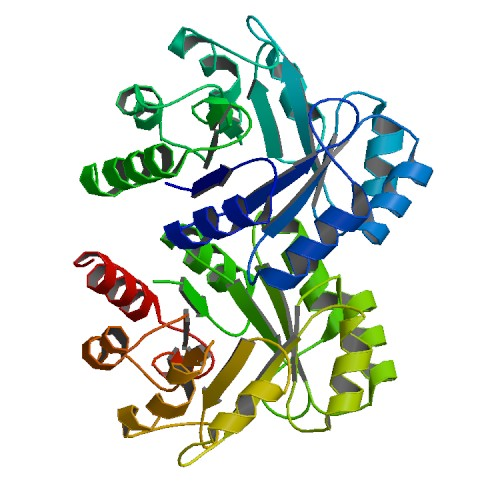
\includegraphics[width=30mm, trim= -10 -5 -5 -10]{1V5X_bio_r_500.jpg} & Topologie: \newline Severin \newline Superfamilie: \newline Severin & Auch dieser Eintrag beschreibt die Struktur einer Phosphoribosyl Anthranilat Isomerase \cite{1v5x}. Hier stammt sie aus \textit{Thermus thermophilus} und ist ebenfalls in die Synthese von L-Tryptophan eingebunden. \\ 
\hline


\end{tabular}
\end{center}
\end{table}

\begin{table}
\begin{center}
\caption{Aldolasen Teil II}
\begin{tabular}{ | C{9mm} | C{30mm} | C{29mm} | C{38mm} | }
\hline
PDB-ID & 3D Bild & Struktur & Beschreibung \\ \hline
1VQT  & 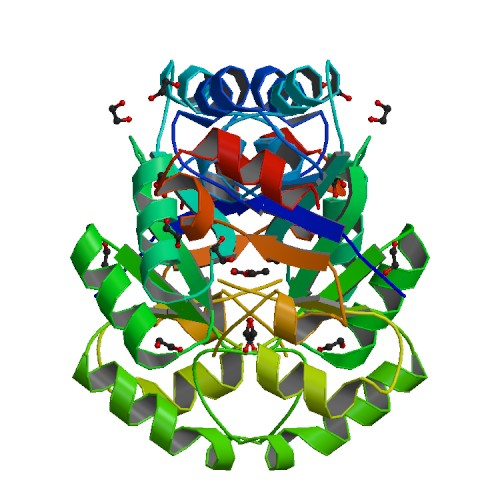
\includegraphics[width=30mm, trim= -10 -5 -5 -10]{1VQT_bio_r_500.jpg} & Topologie: \newline TIM \textit{Barrel} \newline Superfamilie: Aldolasen - Klasse I & Dieser Eintrag beschreibt die Struktur der Oritidin 5'-Phosphatase Decarboxylase aus \textit{Thermotoga maritima} \cite{1vqt}. Sie ist in die Synthese von UMP eingebunden. \\ \hline
1WAU  & 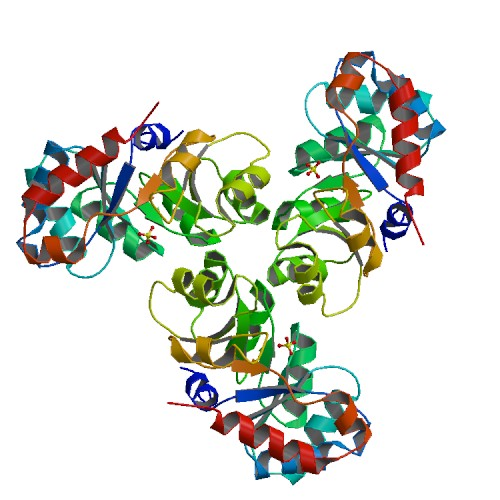
\includegraphics[width=30mm, trim= -10 -5 -5 -10]{1WAU_bio_r_500.jpg} &Topologie: \newline TIM \textit{Barrel} \newline Superfamilie: Aldolasen - Klasse I  & Der Eintrag beschreibt das synthetische Protein T87I phosphono-CheY \cite{2id9}. Es ist ein stabiles Analogon zu dem oben beschriebenen Chemotaxisprotein. \\ \hline
3CEU  & 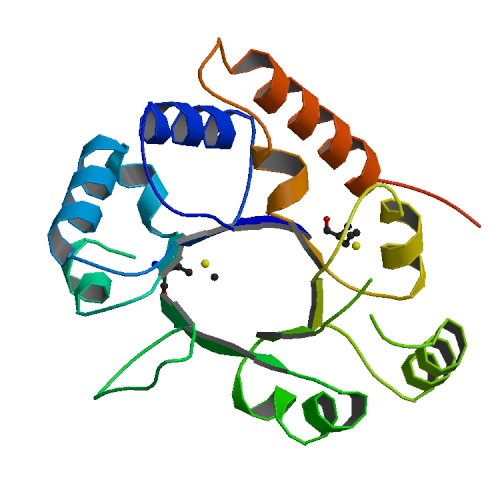
\includegraphics[width=30mm, trim= -10 -5 -5 -10]{3CEU_bio_r_500.jpg}  & Topologie: \newline TIM \textit{Barrel} \newline Superfamilie: Aldolasen - Klasse I & Hier wird die Struktur der E45N Mutante der KDPG-Aldolase aus \textit{E. coli} beschrieben \cite{3ceu}. Das Protein ist in den Glyoxylat und Dicarboxylat Stoffwechsel eingebunden. \\ \hline
7TIM  & 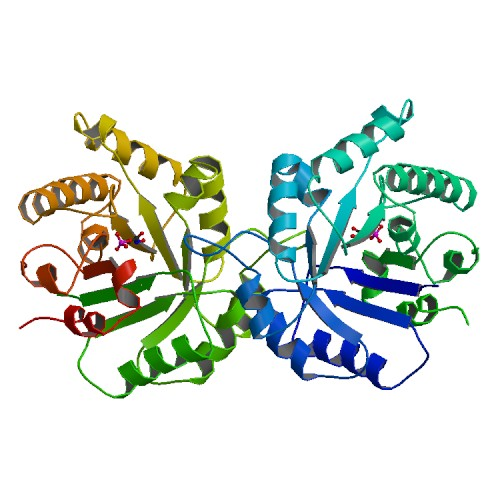
\includegraphics[width=30mm, trim= -10 -5 -5 -10]{7TIM_bio_r_500.jpg} & Topologie: \newline TIM \textit{Barrel} \newline Superfamilie: Aldolasen - Klasse I & Dieser Eintrag beschreibt einen Komplex aus der Triosephosphat Isoermase und Phophoglycolhydroxamat \cite{7tim}. Das Protein ist in die Gluconeogenese eingebunden.\\ 
\hline

% Abkuerzung: KDPG : 2-Keto-3-deoxy-phosphogluconate aldolase

\end{tabular}
\end{center}
\end{table}





\bibliographystyle{plain}
\bibliography{pdb_literatur}


\end{document}